%\documentstyle[aas2pp4,epsf]{article}
%%%\documentstyle[aaspp4,epsf]{article}
%\documentstyle[12pt,aasms]{article}    % this is for a preprint
%(single-spaced)
%\documentstyle[aaspp4,epsf]{article} % this is for small print
%\documentstyle[12pt, aaspp4]{article}

%\documentstyle[11pt,aaspp]{article}
\documentclass[12pt, preprint]{aastex} 

%\documentclass[manuscript]{aastex}
%\documentclass[apj]{emulateapj}

%\documentclass[12pt, preprint,numberedappendix]{emulateapj}
%\documentstyle[12pt,aasms]{article}    % this is for submittal
                                       % (double-spaced)

%\documentstyle[12pt,aasms]{article}   \usepackage{emulateapj5} 

\usepackage{graphicx} 
\usepackage{amsmath}
\usepackage{hyperref}
\usepackage{amsfonts}
\usepackage{amsmath}
\usepackage{amssymb}
\usepackage{amsthm}
\usepackage{subeqnarray}
\usepackage{ulem}
%\bibliographystyle{apj}

\newcommand{\delad}{\nabla_{\rm ad}}
\newcommand{\delrad}{\nabla_{\rm rad}}
\newcommand{\emgr}[1]{\emph{ \color{gray} #1}}

\newcommand{\ie}{i.e.\ }
\newcommand{\eg}{e.g.\ }
\newcommand{\p}{\partial}
\newcommand{\xv}{\vc{x}}
\newcommand{\kv}{\vc{k}}
\newcommand{\brak}[1]{\langle #1\rangle}


\newcommand{\gcc}{\;\mathrm{g\; cm^{-3}}}
\newcommand{\gsc}{\;\mathrm{g\; cm^{-2}}}
\newcommand{\cm}{\; {\rm cm}}
\newcommand{\mm}{\; {\rm mm}}
%\newcommand{\ps}{\; {\rm s^{-1}}}
\newcommand{\km}{\; {\rm km}}
%\newcommand{\au}{\; \varpi_{\rm AU}}

\newcommand{\AU}{\; {\rm AU}}
\newcommand{\yr}{\; {\rm yr}}
\def\K{\; {\rm K}}

\newcommand{\vcs}[1]{\mbox{\boldmath{$\scriptstyle{#1}$}}}
\newcommand{\vc}[1]{\mbox{\boldmath{$#1$}}}
\newcommand{\nab}{\vc{\nabla}}
\DeclareMathSymbol{\varOmega}{\mathord}{letters}{"0A}
\DeclareMathSymbol{\varSigma}{\mathord}{letters}{"06}
\DeclareMathSymbol{\varPsi}{\mathord}{letters}{"09}

\newcommand{\Eq}[1]{Equation\,(\ref{#1})}
\newcommand{\Eqs}[2]{Equations (\ref{#1}) and~(\ref{#2})}
\newcommand{\Eqss}[2]{Equations (\ref{#1})--(\ref{#2})}
\newcommand{\Eqsss}[3]{Equations (\ref{#1}), (\ref{#2}) and~(\ref{#3})}
\newcommand{\App}[1]{Appendix~\ref{#1}}
\newcommand{\Sec}[1]{Sect.~\ref{#1}}
\newcommand{\Chap}[1]{Chapter~\ref{#1}}
\newcommand{\Fig}[1]{Fig.~\ref{#1}}
\newcommand{\Figs}[2]{Figs.~\ref{#1} and \ref{#2}}
\newcommand{\Figss}[2]{Figs.~\ref{#1}--\ref{#2}} 
\newcommand{\Tab}[1]{Table \ref{#1}}

\newenvironment{packed_item}{
\begin{itemize}
  \setlength{\itemsep}{1pt}
  \setlength{\parskip}{0pt}
  \setlength{\parsep}{0pt}
}{\end{itemize}}

%\newcommand{\delad}{\nabla_{\rm ad}}
%\newcommand{\delrad}{\nabla_{\rm rad}}
\newcommand{\Rg}{\mathcal{R}}
\newcommand{\RB}{R_{\rm B}}
\newcommand{\co}{_{\rm c}}
\newcommand{\di}{_{\rm d}}
\newcommand{\cb}{_{\rm RCB}}
\newcommand{\surf}{_M}
\newcommand{\mc}{m_{\rm c \oplus}}
\newcommand{\mcn}[1] { m_{ \rm c #1 \oplus} }
\newcommand{\MC}{M_{\rm crit}}
\newcommand{\au}{a_\oplus}
\newcommand{\aun}[1]{ a_{#1\oplus} }

\begin{document}
\bibliographystyle{apj}

\title{The Influence of Radial Drift and Gas Accretion on the C/O Ratio in Protoplanetary Disks}

The chemical composition of giant planet atmospheres can provide important constraints on the formation of these planets, as well as on their accretion and migration history. An important signature of atmospheric chemistry in giant planets is the C/O ratio. The C/O ratio has been estimated observationally in some giant planets, and it has been found to be different than the solar C/O ratio of the host star \citep{madhu11}. One explanation for this difference was proposed by \citet{oberg11}. Their basic idea was that the main carriers of carbon and oxygen, i.e. H$_2$O, CO$_2$ and CO, have different condensation temperatures. This results in variations in the abundances of C and O in solids and gas between the snow lines of the volatiles mentioned above. Figure \ref{fig:CtoO} shows the C/O ratios in the gas and in the dust as a function of semimajor axis, for a passively irradiated disk. As a fiducial disk model we choose the prescription of \citet{chiang10} for the gas temperature and surface density profile:

\begin{eqnarray}
\label{eq:diskmodel}
T_{\rm d} = 120 \times (a/\rm AU)^{-3/7} \,\,\, \rm K \\
\Sigma_{\rm d} = 2000 \times (a/\rm AU)^{-1} \,\,\, \rm{g \, cm}^{-2},
\end{eqnarray}
where $a$ is the semimajor axis.


\begin{figure}[htb]
\centering
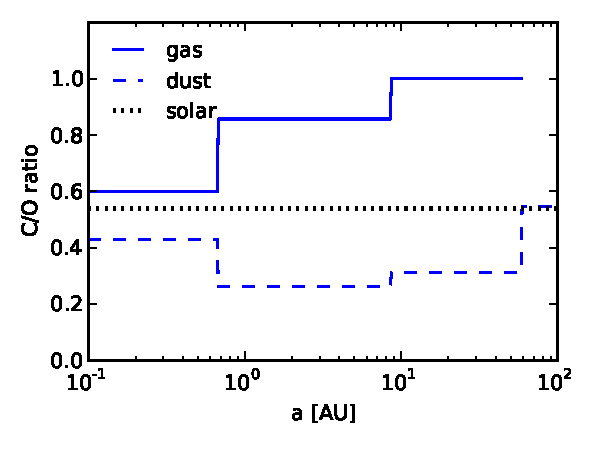
\includegraphics[width=0.8\textwidth]{../figs/C_O_ratio_2.pdf}
%\vspace{-0.5in}
\caption{C/O ratio in gas and in dust as a function of distance, for a passively irradiated protoplanetary disk (see Equation \ref{eq:diskmodel}). After \citet{oberg11}.} %  (See text for a description of evolution to yet higher masses.) 
\label{fig:CtoO}
\end{figure}

Starting from the premise of \citet{oberg11}, our long-term goal is to investigate the various chemical and dynamical processes that take place in protoplanetary disks, and understand which of this processes are relevant for the chemical variations in the atmospheres of gas giants, and under which conditions. We begin by studying the effect of the radial drift of solids on the location and shape of snowlines in disks.  

\section{Radial Drift}

Solids planetesimals in disks orbit their host star at a Keplerian velocity. The gas, on the other hand, experiences an extra pressure gradient, which causes it to rotate at a sub-Keplerian velocity. Thus solid particles experience a headwind, which tends to remove angular momentum and cause the planetesimals to spiral inwards and fall into the host star. Small planetesimals are well-coupled to the gas, so they rotate with the gas at the sub-Keplerian frequency and their drift timescales are very large compared to the lifetime of the gas disk. Conversely, large planetesimals are decoupled from the gas, thus the influence of gas drag on them is negligible and their radial drift times also exceed the disk lifetime. On the other hand, planetesimals of intermediate sizes ($\sim$0.1cm - $\sim$10 km, depending on their location and the disk temperature and surface density profile) can have short drift timescales relative to the disk lifetime. This is shown in Figure \ref{fig:drift_times} at the H$_2$O, CO$_2$ and CO snowlines, respectively. The plot also shows the desorption (or evaporation) timescale as a function of particles size at the same stellocentric distances. We thus see that, if the drift timescale is shorter than the evaporation timescale, planetesimals might drift a significant distance past a given snowline before they desorb. This therefore changes the location and shape of snowlines, and thus the C/O ratio from the profile depicted in Figure \ref{fig:CtoO}.

\begin{figure}[htb]
\centering
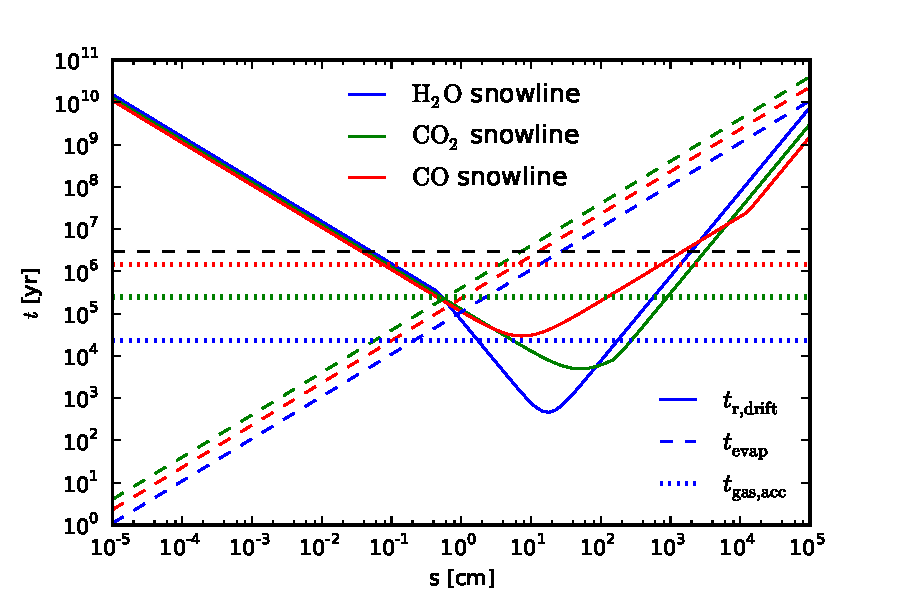
\includegraphics[width=0.8\textwidth]{../figs/drift_timescales_betaS1_gas_acc.pdf}
%\vspace{-0.5in}
\caption{Drift timescale (solid lines), desorption timescale (dashed lines), and gas accretion timescale for $\alpha=0.01$ (dotted lines) as a function of particle size, at three representative locations: the H$_2$O snowline (in blue), the CO$_2$ snowline (in green) and the CO snowline (in red). The horizontal dashed black line shows a typical disk lifetime of 3 Myr.} %  (See text for a description of evolution to yet higher masses.) 
\label{fig:drift_times}
\end{figure}

\begin{figure}[htb]
\centering
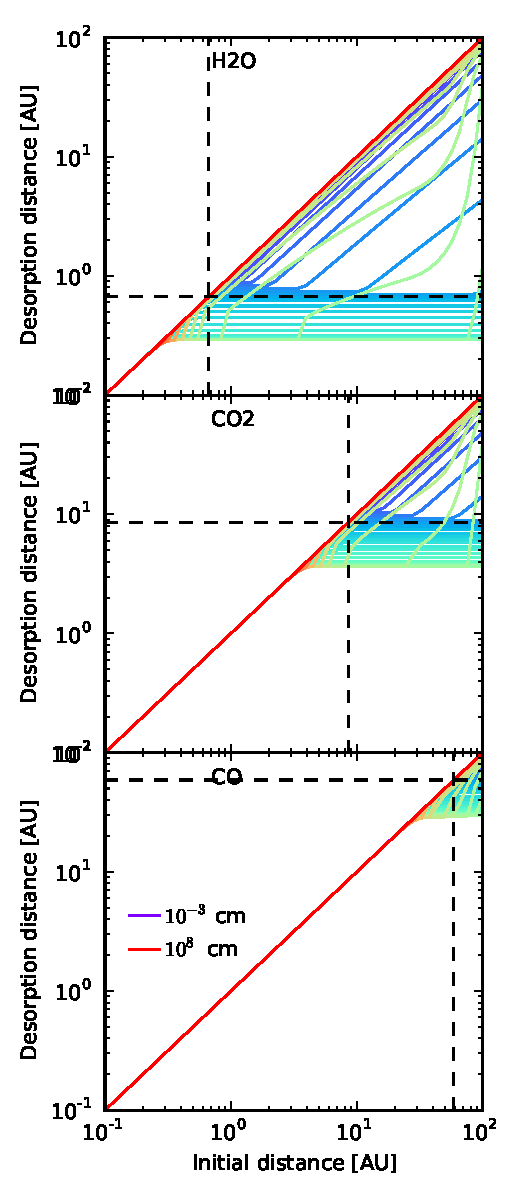
\includegraphics[width=0.5\textwidth]{../figs/desorption_distance_many_new_2.pdf}
%\vspace{-0.5in}
\caption{Desorption distance as a function on initial particle distance for H$_2$O (top panel), CO$_2$ (middle panel) and CO (bottom panel), for particle size between $10^{-3}$ and $10^8$ cm. The vertical and horizontal dashed lines show the respective snowlines as calculated based on \citet{hollenbach09}. Small particles desorb instantaneously, while large particles do not either drift or desorb before disk dissipation. Intermediate size planetesimals desorb at a fixed distance that depends on the particle size, regardless of their initial location in the disk.} %  (See text for a description of evolution to yet higher masses.) 
\label{fig:drift_dist}
\end{figure}

\begin{figure}[htb]
\centering
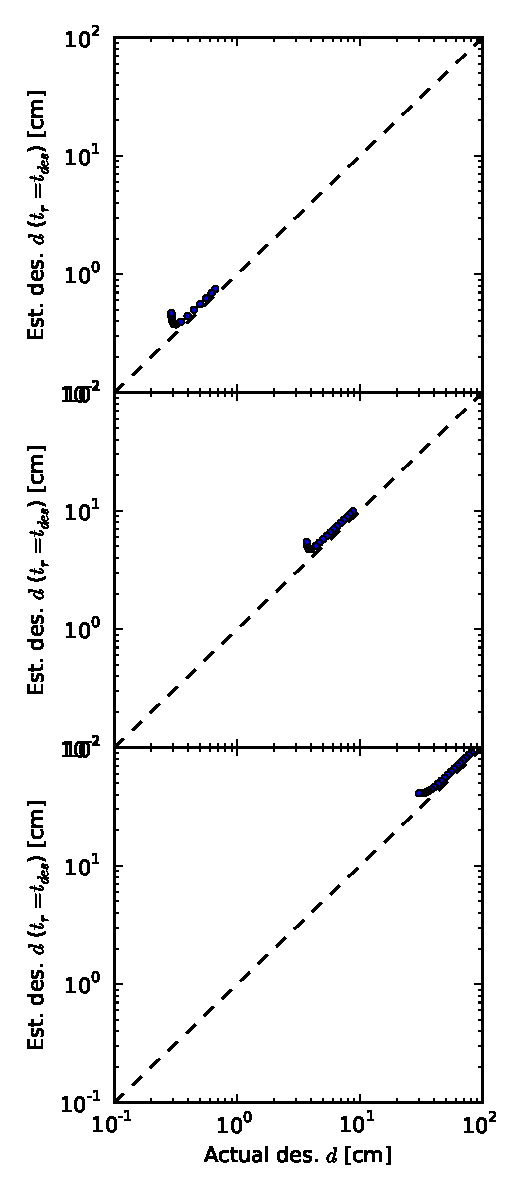
\includegraphics[width=0.5\textwidth]{../figs/desorption_distance_actual_vs_estimated.pdf}
%\vspace{-0.5in}
\caption{Desorption distance estimated analytically (when the drift and desorption times are equal) versus the desorption distance calculated numerically, for H$_2$O (top panel), CO$_2$ (middle panel) and CO (bottom panel), and for different initial particle sizes. The analytic and numerical results are in good agreement.} %  (See text for a description of evolution to yet higher masses.) 
\label{fig:an_vs_num}
\end{figure}

\begin{figure}[htb]
\centering
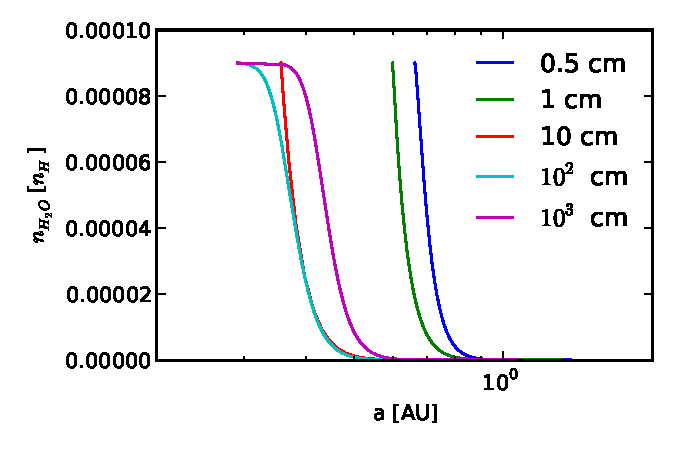
\includegraphics[width=0.8\textwidth]{../figs/nH2O_no_acc.pdf}
%\vspace{-0.5in}
\caption{Abundance of water vapor with respect to Hydrogen as a function of semimajor axis, for various particle sizes. Radial drift changes both the shape and the location of the H$_2$O snowline.} %  (See text for a description of evolution to yet higher masses.) 
\label{fig:nwater_drift}
\end{figure}

We calculate self-consistently the drift and desorption distances as a function of particle size for our fiducial disk. We calculate the desorption rates following the prescription of \citet{hollenbach09}, assuming that the solids are perfect spheres and composed of a single volatile material (either H$_2$O, CO$_2$ or CO). To calculate the drift timescale, we follow the analytic prescription of \citet{chiang10}. We integrate the drift and desorption equations self-consistently, and stop the evolution at $\tau=3$ Myr, the typical lifetime of a protoplanetary disk. 


Figure \ref{fig:drift_dist} shows the desorption distance as a function of the initial planetesimal location, for H$_2$O, CO$_2$ and CO particles. As expected, small planetesimals desorb instantly, while large boulders do not have enough time to either desorb or drift before the disk dissipates. We notice, however, that planetesimals with sizes between $\sim 1$ cm and $\sim 10^3$ cm, desorb at a fixed distance from the host star, regardless of their initial location in the disk. This desorption distance depends on the planetesimal size. We have found that this distance can be well approximated analytically as the radius at which the desorption and drift timescales are equal (see Figure \ref{fig:an_vs_num}). Figure \ref{fig:nwater_drift} shows the abundance of H$_2$O with respect to Hydrogen as a function of semimajor axis. We see that particles evaporate most of their mass at their desorption distance (see Figure \ref{fig:drift_dist}). 



Our drift calculation shows that the location of snowlines is not fixed, but rather dependent on planetesimal size. So far in our calculations we have assumed a passively irradiated disk. However, observations have shown that young Sun-like stars actively accrete gas from the disk at typical rates $\dot{M}_{\rm gas} \sim 10^{-8}$ $M_{\odot}$/year (e.g., \citealt{hartmann06}). The abundance of H$_2$O, CO$_2$ and CO in gas and grains, and therefore the C/O ratio in gas, will depend on the relative mass accretion rates of solids (due to drift) and of gas (due to viscosity).

For simplicity we first assume a constant gas accretion rate, $\dot{M}_{\rm gas}=-2 \pi a \dot{a_{\rm g}} \Sigma_{\rm d}$ , where $\dot{a}_{\rm g}$ is the radial velocity of the gas and $\Sigma_{\rm d}$ is given by Equation (\ref{eq:diskmodel}). The mass accretion rate of the drifting solids can be calculated as $\dot{M}_{\rm solids} = - 2 \pi a \dot{a}_{\rm drift} \Sigma_{\rm p}$, where $\dot{a}_{\rm drift}$ is the drift velocity of planetesimals (see \citealt{chiang10}, Equation 13 for an expression) and $\Sigma_{\rm p}$ is the surface density of solids. We assume a dust to gas ratio of 0.01, i.e. $\Sigma_{\rm d}=100 \Sigma_{\rm p}$. 

\textbf{This is where it gets tricky, because my plot is obviously wrong (see below). Basically, I am starting with the simplest case: I'm assuming I have only one H$_2$O particle size (in this case $s=1$ cm), at an initial distance of 10 AU. My thinking was the following: the ratio between the abundance of H$_2$O in solids and the gas abundance in the disk should just be given by the ratio between the mass fluxes of solids and gas. So for a given $a$ and $s$, $n_{\rm H_2 O, solids}/n_{\rm H} = \dot{M}_{\rm solids}/\dot{M}_{\rm gas}$. Then $n_{\rm H_2 O, gas}/n_{\rm H} = 1-n_{\rm H_2 O, solids}/n_{\rm H}=1-\dot{M}_{\rm solids}/\dot{M}_{\rm gas}$. Then I multiply this by the total water abundance with respect to Hydrogen, i.e. $0.9 \times 10^{-4}$ from \citet{oberg11}. However, I am pretty sure this is wrong. First off, I don't get the results from Figure \ref{fig:nwater_drift} for $\dot{M}_{\rm gas}=0$. Figure \ref{fig:wrong} is also wrong, starting with the fact that $n_{\rm H_2 O} \neq 0$ at 10 AU, as it should. Hopefully we can discuss this during our Skype call --- I'm fairly sure it shouldn't be too complicated and I'm missing something obvious, but haven't figured out what so far.}

\begin{figure}[htb]
\centering
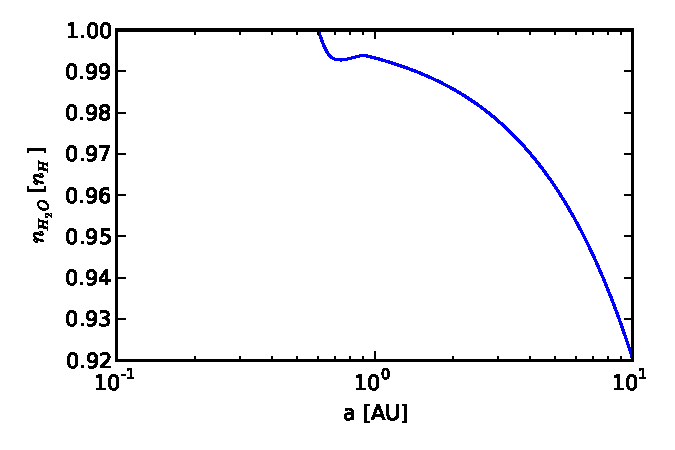
\includegraphics[width=0.8\textwidth]{../figs/nH2O_acc_wrong.pdf}
%\vspace{-0.5in}
\caption{Attempt to show the abundance of water vapor with respect to Hydrogen as a function of semimajor axis for one particle size, when both drift and gas accretion are included. Obviously wrong.} %  (See text for a description of evolution to yet higher masses.) 
\label{fig:wrong}
\end{figure}


\section{TO DO NEXT}

\begin{itemize}
\item Calculate C/O ratios assuming a particle size distribution --- $n \sim s^{-2.5}$ seems reasonable, but see Til's 2011/2012 papers for better estimates.
\item Add particle growth into the drift calculation --- see Til's 2012 paper for an analytic estimate of growth rates; in principle it should be relatively straightforward, just need to add an extra differential equation in the drift + desorption evolution.
\item Calculate abundances and C/O ratios for different disk models; perhaps also use the temperature profile for an actively accreting disk, for consistency with the assumption of constant $\dot{M}_{\rm gas}$?
\item Discuss turbulence --- we had decided through qualitative arguments that it shouldn't matter, but we need to formulate it more rigorously.
\item Perhaps show snapshots of C/O ratio plots at different times in the disk evolution, not just after gas dissipation at 3 Myrs?
\item Discuss how good the sphere approximation is for the grains --- see the paper links that Til sent us.
\item Include also $\rm N_2$? Might be too much for this paper... 
\end{itemize}
     



\bibliographystyle{apj}
\bibliography{refs}

\end{document}
